\documentclass[12 pt,a4paper,frenchb]{article}

\usepackage{babel}

\usepackage{graphicx}
\graphicspath{{images/}}

\usepackage{titling}

\usepackage{url}

\usepackage[T1]{fontenc}
\usepackage{fontspec}

\usepackage[french]{algorithm2e}
\SetKwInput{Donnees}{Données}
\SetKwInput{Res}{Résultats}
\SetKwIF{Si}{SinonSi}{Sinon}{si}{alors}{sinon si}{alors}{finsi}
\SetKwFor{Tq}{tant que}{faire}{fintq}

\setlength{\parindent}{4em}
\setlength{\parskip}{1em}

\title{Rapport du projet MyAdblock}
\author{Adam FACI \\ Quentin DECHAUX}
\date{25 Avril 2017}

\begin{document}

\begin{titlingpage}
  
\includegraphics[scale = 0.6]{TNCY.jpg}
  
\includegraphics[scale = 1.2]{UL.jpg}
  \begin{center}
    \vspace{4cm}
    \textbf{\Huge{\thetitle}}\par
    \vspace{1.5cm}
    \theauthor\par
    \vspace{2cm}
    \thedate
    \vspace{4cm}
  \end{center}
  \textbf{Cours :} Réseaux et Systèmes Avancés : Partie Réseaux\\
  \textbf{Professeur :} Isabelle CHRISMENT
\end{titlingpage}

\tableofcontents
\thispagestyle{empty}

\newpage
\setcounter{page}{1}

\section{Introduction}

Projet effectué dans le cadre du cours de RSA visant à comprendre la notion de serveur proxy HTTP en créant le nôtre et en l'utilisant en tant que \textbf{AdBlock} ie. en tant que bloqueur de publicités.

Le serveur devra à chaque requête arrivant sur notre machine vérifier que l'hôte de celle-ci ne fait pas partie d'une liste prédéfinie de serveurs de publicités.

À priori la liste proviendra du site \url{https://easylist.to/}.

\section{Analyse des échanges TCP et HTTP entre un client et un serveur}

\subsection{Analyse des échanges sans proxy}

Pour cette analyse, nous nous sommes juste connectés au site \url{www.telecomnancy.net}. Afin de repérer la conversation sur wireshark, nous avons d'abord filtré avec \textbf{http} afin de repérer plus facilement dans la colonne info un \textit{GET / HTTP/1.1}. Une fois trouvé, nous avons isolé les échanges via un filtre plus précis.

Les échanges TCP et HTTP entre le client (notre machine) et le serveur web (le site \url{www.telecomnancy.eu}) ont ainsi été triés via le filtre : \textbf{tcp \&\& ip.addr == 193.54.21.201} où \textbf{193.54.21.201} correspond à l'adresse ip du site au moment de la communication et la condition \textbf{ip.addr == 193.54.21.201} exige que l'adresse soit présente dans la trace (en source ou destinataire). Aussi, la condition \textbf{tcp} impose qu'un en-tête TCP soit présent, ce qui est le cas pour les traces TCP et HTTP.

Le résultat de ces échanges sont en pièce jointe dans le fichier 
\og\textit{capture\_file\_question\_1.pcapng}\fg.

Cela commence tout d'abord avec un \textit{TCP three-way handshake} avec le serveur qui reçoit le segment SYN, nous qui recevons le segment SYN+ACK et enfin le serveur qui reçoit le segment ACK.

\begin{figure}[h]
  \centering
  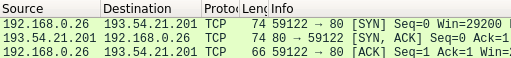
\includegraphics[height=2.5cm,width=15cm]{Q1/three_way_handshake.png}
  \caption{Le three-way handshake}
\end{figure}
\vspace{1cm}

Cela correspond à l'établissement de la connexion entre le client et le serveur.

Ensuite, un paquet HTTP est envoyé au serveur avec pour en-tête HTTP \textit{GET / HTTP/1.1}.
\vspace{1cm}

\begin{figure}[h]
  \centering
  \includegraphics{Q1/requête_HTTP.png}
  \caption{Requête HTTP au serveur}
\end{figure}
\vspace{1cm}

Il correspond à la demande du contenu de la page d'accueil du site web par le client. Il contient les données TCP avec l'en-tête HTTP au dessus.

Ensuite le client reçoit deux paquets : un paquet TCP et un paquet HTTP.
\vspace{1cm}

\begin{figure}[h]
  \centering
  \includegraphics[scale=0.8]{Q1/réponse_serveur.png}
  \caption{La réponse du serveur}
\end{figure}
\vspace{1cm}

Le paquet TCP correspond à l'acquitement de la requête HTTP précédente. Le paquet HTTP correspond quant à lui à la réponse à la requête HTTP du client. Elle spécifie une redirection avec la mention \textit{Moved Permanently} accompagné d'un contenu html.

\begin{figure}[h]
  \centering
  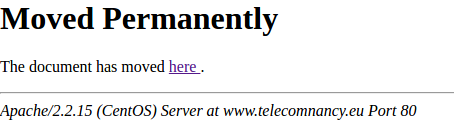
\includegraphics[scale=0.8]{Q1/contenu_html.png}
  \caption{Le contenu html de la réponse}
\end{figure}
\vspace{1cm}

Cela est dû au fait que le site de l'école est en désormais hébergé à l'adresse \url{www.telecomnancy.univ-lorraine.fr}. En réalité, lors de la navigation sur le site web, rien n'est affiché et la redirection est automatique.

Puis un acquittement de la réponse est envoyé par le client au serveur via un paquet TCP.


\begin{figure}[h]
  \centering
  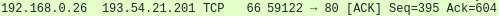
\includegraphics{Q1/acquittement_final.png}
  \caption{L'acquitement de la réponse}
\end{figure}
\vspace{1cm}

À noter que selon les essais, et selon que nous allions sur différentes page du site ou nous, certains échanges supplémentaires avec d'autres serveurs comprenant des fichiers supplémentaires nécessaires comme des feuilles de style en cascade (.css) , des établissement de connexions (\textit{TCP three-way handshake}), ou des requêtes jQuery (pour un affichage rapide et dynamique des éléments de la page web).


\subsection{Mise en place du proxy}

Nous devons ensuite effectuer la même analyse avec l'utilisation d'un serveur proxy.

Pour cela, nous avons cherché un proxy gratuit, et sommes tombé sur un proxy qui nous faisait passer par l'Allemagne afin que le site demadé nous localise là-bas. Voulant travailler sur le plus simple possible, nous avons encore cherché et avons finalement opté pour le proxy proposé sur le site \url{www.simpleproxy.net}.

Diverses options étaient disponibles comme la possiblité de crypter l'URL demandée ou de refuser les scritps (ajax par exemple), mais encore une fois nous avons tous décoché. Les résultats obtenus sont donnés dans la section suivante.

\subsection{Analyse des échanges avec proxy}

Lors de cette analyse, nous sommes donc allés sur le site du proxy, puis nous avons une fois de plus demandé à atteindre le site \url{www.telecomnancy.eu} avant de couper la connexion.

Nous avons cherché la conversation de la même façon que précédemment et sommes très vite tombé sur la requête HTTP ayant pour info  \textit{GET \textbackslash browse.php?u=http\%3A\%2F\%2Ftelecomnancy.univ-lorraine.fr\&b=4}. Afin d'isoler la conversation sur wireshark, nous avons alors appliqué le filtre \textbf{tcp.port == 51276} car le port \textbf{51276} correspondait à tous les paquets de la conversation. De plus ce filtre implique également de n'avoir que des paquets comprenant un en-tête TCP. Aussi, un port restant exclusif à une seule communication, cela nous assure également que les traces y venant et en sortant dont bien avec le même interlocuteur.

Au début de la conversation, on constate de la même façon un \textit{three way handshake} correspondant à l'établissement de la connexion au site via le proxy.

\begin{figure}[h]
  \centering
  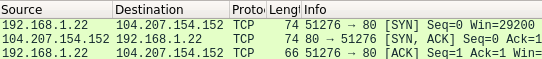
\includegraphics[scale=0.8]{Q3/three_way_handshake.png}
  \caption{Le three way handshake}
\end{figure}
\vspace{1cm}

Puis il y a une première requête HTTP du site qui renvoie un paquet malformé. Puis un second essai avec cette fois une série de dizaines de paquets échangés avec des données arrivant et un acquittement en réponse.

\begin{figure}[h]
  \centering
  \includegraphics{Q3/requête_HTTP.png}
  \caption{Première requête HTTP}
  \vspace{1cm}
  \includegraphics{Q3/réponse_serveur.png}
  \caption{Réponse du serveur}
  \vspace{1cm}
  \includegraphics{Q3/requête_HTTP_2.png}
  \caption{Deuxième requête HTTP}
\end{figure}
\vspace{1cm}

Par la suite, contrairement à la situation sans proxy, il y a un échange d'une série de paquets TCP entre le client et le serveur, correspondant aux données de la page à charger. Cela doit être dû à la mauvaise connexion à cause du passage par le proxy.

Enfin lorsque nous quittons le site, contrairement à la première fois, le proxy prend le temps d'effectuer une fermeture de connexion via l'établissement d'un échange de paquets TCP ayant les flags \textit{FIN} activés.

\begin{figure}[h]
  \centering
  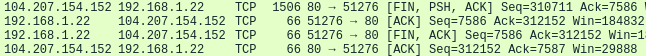
\includegraphics{Q3/fin_de_connexion.png}
  \caption{Fin de connexion}
\end{figure}
\vspace{1cm}

\section{Notre proxy}

\subsection{Spécification de l'algorithme}

Nous allons détailler ici une première approche de l'algorithme de notre serveur proxy en pseudo-code.

\begin{algorithm}[h]
  \Donnees{RequêteClient, RéponseServeur, SocketClient, SocketServeur, AdresseServeur}
  \Res{Laisse passer la RéponseServeur au client ou lui renvoie une erreur}
  \Tq{Serveur Proxy Lancé}{   
    //ie tant que le serveur proxy est en ligne.\par
    Attente de l'arrivée d'une requête\; 
    //ie d'une requête par un client.\par
    \Si{Requête arrivée}{ 
      //Si une requête est réceptionnée au niveau du socket\par
      RequêteClient = RécupérerRequête(SocketClient)\;
      AdresseServeur = RequêteToAdresse(RequêteClient)\; 
      //Récupère l'adresse demandée dans la requête\par
      \Si{not AdresseOK(AdresseServeur)}{ 
        //On teste si l'adresse est interdite ou pas.\par
        AfficherDansLaConsole(\og L'adresse \%s est bloquée par le proxy.\fg,AdresseServeur)\;
      }
      \Sinon{
        SocketServeur = CréerSocket(AdresseServeur)\;
        EnvoyerRequête(RequêteClient,SocketServeur)\;
        RéponseServeurTemp = 0\; 
        //Variable locale qui sockera les paquets reçus au fur et à mesure.\par
        \Tq{not RéponseServeur}{ 
          //Tant que la Réponse du serveur n'est pas définie.\par
          RéponseServeurTemp += RécupérerRéponse(SocketServeur)\; 
          //On récupère le paquet envoyé par le serveur.\par
          TailleDonnéesRestantes = RéponseServeurTemp.TailleDonnéesRestantes\;  
          //On récupère dans les flags la taille des données restantes.\par
          \Si{TailleDonnéesRestantes == 0}{ 
            //ie le dernier paquet a été reçu.\par
            RéponseServeur = RéponseServeurTemp\;
            Fermer(SocketServeur)\;
          }
        }
        RetourneRéponse(SocketClient)\;
      }
    }
  }
  \caption{Algorithme du proxy}
\end{algorithm}



\end{document}